% !TeX root = ../main.tex

\chapter{系统设计与实现}

本章设计并实现了一个具有交互性和用户友好性的基于知识图谱和大语言模型智能体机制的API编排和调用系统。该系统集成了不同模型的调用接口,以及知识图谱查询的功能。该系统提供了一个使用门槛低、用户友好的界面,允许用户通过自然语言的方式与该系统进行交互和提问,系统会根据用户的需求编排并调用所需的API,并进行回答。

难点:

界面设计:友好交互、展示图谱部分、添加api部分

前后端框架选什么

前:streamlit 后:fastapi


模型管理(不同模型,超参数,上下线) 如何交互 容错 restapi格式 如何加速

数据管理 neo4j qdrant 用户数据 记忆数据

\section{系统需求分析}

\indent 我们采用面向对象的需求分析方法,绘制了如图所示的系统用例图。

“如图~\ref{fig:usecase} 所示”等。该页空
白不够排写该图整体时,则可将其后文字部分提前排写,将图移到次页。

\begin{figure}[!htp]
  \vspace{1em}
  \centering
  \setlength{\abovecaptionskip}{10pt} % 控制图片和caption之间的距离
  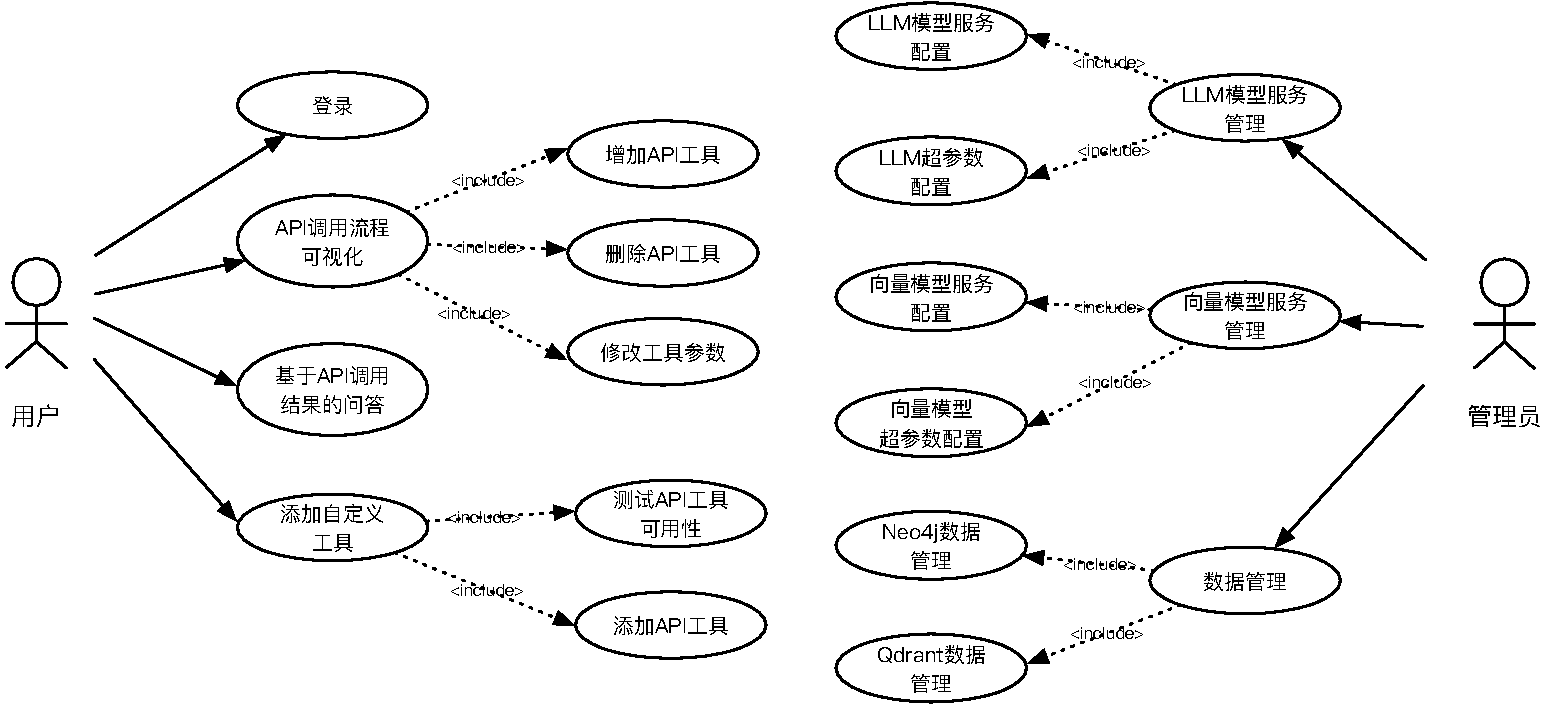
\includegraphics[height=7cm]{../assets/ch5-用例图.pdf}
  \bicaption{系统用例图}{System Usecase Diagram}
  \label{fig:usecase}
\end{figure}

在用例图中,我们定义了两种角色:系统用户和管理人员。从需求出发,系统应该实现以下功能:

针对普通用户的功能:

1. 登录功能

2. API调用流程可视化

3. 基于API调用结果的问答

4. 添加自定义工具

针对管理员的功能:

1. 大语言模型服务管理

2. 向量模型服务管理

3. 数据管理

在该系统中,基于大语言模型的智能体可以通过多轮对话的交互方式与用户进行交流,并通过解析用户的需求来提供对应的工具调用流程和根据工具调用结果得到的总结回复

本文的系统提供的主要功能是根据用户需求得到调用流程并执行,从而给用户提供有效的信息。针对该核心功能,我们针对不同用户群体设计了两种使用的模式:对于有计算机编程基础的用户,我们提供了开发者模式,即用户可以自己对工具执行流程进行编辑和调整,以确保更加符合其查询需求;对于一般用户,我们按照系统生成的流程进行执行,得到最终结果。除了该功能外,本系统还提供了自定义工具添加、工具模板库浏览等功能。

\section{系统设计与架构}
本文设计的基于知识图谱和智能体的API编排与调用系统,整体的系统框架设计如图xx所示。系统主要包含四层:数据管理层、API编排层、API调用层和UI层。

\subsection{交互方案设计}


\subsection{系统架构设计}

\indent 本系统的架构将会从部署架构和软件架构来进行说明。

部署架构。

软件架构。


\subsection{数据管理层}
数据管理层主要负责下列内容的存储:
\begin{enumerate}
    \item API知识图谱的存储
    \item 向量形式存储的API详细信息,这些预先计算并存储在向量数据库中,便于快速计算
    \item 系统使用过程中的历史推理轨迹的存储,作为经验数据供后续参考
\end{enumerate}

\subsection{API编排层}
API编排层主要实现本系统的动态API编排功能。该层主要包括以下几个部分:
\begin{enumerate}
    \item \textbf{用户需求拆解模块}:通过大语言模型智能体机制,将用户的复杂、完整需求拆解为多个子需求,并对子需求逐一调用。
    \item \textbf{API推理轨迹检索模块}:根据子任务的任务描述,检索历史推理轨迹中相似任务,提供参考。
    \item \textbf{API知识图谱检索模块}:根据不同的检索模式,搜索API节点及相关信息作为返回。
    \item \textbf{基于图谱的DFS动态编排算法模块}:在知识图谱上进行搜索和回溯,得到最终的调用路径。
\end{enumerate}
该层的主要流程为:首先通过拆解模块将任务拆解为独立的子任务,然后针对每个子任务,检索类似任务作为参考,并检索相关API信息,构建提示词,基于大模型的推理能力和上下文生成结构化的API流程。

\subsection{API调用层}
API调用层主要负责根据API编排层生成的调用流程,获取调用参数并执行API调用。主要涉及到以下部分:
\begin{itemize}
    \item \textbf{API参数获取模块}: 首先,我们获取得到对应API的参数信息以及用户的具体需求,提供给大语言模型让模型给出API所需的输入参数。
    \item \textbf{API调用模块}: 在该部分,会使用API参数获取模块的参数作为API输入来调用工具API,若执行成功则将JSON格式的调用结果传递到API调用结果总结模块。该部分设置了自动重试机制,若调用失败则自动重试3次,如果3次都失败则返回错误信息。
    \item \textbf{API调用结果总结模块}: 在执行并得到了API的调用结果后,将所有的API执行结果转化为自然语言的格式,将这些执行结果和用户原需求输入基于大语言模型的总结模块获取最终自然语言格式的总结内容。
\end{itemize}

\subsection{UI层}
UI层是web前端页面,负责与用户直接交互,提供用户友好的界面。不同页面对应不同功能:
\begin{itemize}
    \item \textbf{信息问答页面}:用户通过自然语言输入具体的需求,然后系统会进行API调用路径的编排并依次调用,最终将总结好的自然语言文本的结果也提供给用户。整体的交互方式与大模型多轮对话是相似的。
    \item \textbf{自定义API添加页面}:用户可以通过填写API的详细信息,如API的名称、API的调用链接、API的具体参数类型和参数描述信息等添加新的API。添加新API后还需要经过测试,确保API调用的有效性再添加到API仓库中。
    \item \textbf{API历史调用参考页面}:用户可以可视化的形式浏览历史API调用记录,并通过选择和配置参数的方式再次调用历史API调用链。
\end{itemize}
UI层代码是基于streamlit代码库实现的。

\subsection{数据库设计}

画er图。

\subsection{模块设计}

图xx展示了系统详细的功能层次结构。本系统的详细功能主要包含:用户验证、数据管理、模型服务管理、API工作流编排、API调用问答、自定义API存储。

\subsection{用户验证}
用户验证模块用于实现面向用户的API调用历史记录和模板库构建。该模块包含用户注册和登录功能,允许用户通过注册获得个人账号并登录系统使用。

\subsection{数据管理}
数据管理模块用于管理系统中的各类数据,包括知识图谱数据、API信息向量以及用户交互过程中的历史需求、API编排和调用结果等。主要存储在neo4j和Qdrant向量数据库中。

\subsection{模型服务管理}
模型服务管理模块包括模型接口封装和模型超参数配置功能。封装不同模型的调用代码为统一接口,对系统其他部分隐藏模型的具体细节。超参数配置则管理模型调用时的参数,如温度系数、最大长度、top\_k、top\_p等。

\subsection{API工作流编排}
API工作流编排模块包含以下三个子模块:
\begin{itemize}
    \item \textbf{编排模式选择}:提供用户可配置的编排选项。
    \item \textbf{编排结果展示}:通过可编辑任务框展示API编排结果,任务框中展示API名称、描述、参数等信息。
    \item \textbf{API流程自定义}:允许用户在生成的API流程基础上,进行增加、删除或修改,支持更灵活的API调用。
\end{itemize}

\subsection{API调用问答}
API调用问答模块通过流式输出和多轮交互,提升用户体验。流式输出模块增强用户等待结果时的体验,多轮交互模块保存上下文中的API调用结果,支持进一步提问。

\subsection{自定义API存储}
自定义API存储模块通过API添加和测试模块,支持用户将自定义API添加到系统中,提高系统扩展性和可用性。

\section{系统实现}

技术选型。



\section{系统展示}
(此处为系统截图展示)

\section{本章小结}